
\documentclass{../thesis}

\subtitle{Diplomarbeit}
\title{Algorithmen zur automatisierten Generalisierung durch Zusammenfassung von Linienzügen in OpenStreetMap\\ für konkrete Spezialfälle}
\author{Arne Johannessen}
\publishers{betreut durch\\ Prof. Dr. rer. nat. Detlef Günther-Diringer\\ und\\ Dipl.-Wi.-Ing. Frederik Ramm}
%\date{Arbeitsentwurf}
%\dedication{}

%\ccbysa
% https://creativecommons.org/licenses/by-sa/4.0/legalcode.de
% https://wiki.creativecommons.org/wiki/License_Versions
% ODBL: 2009 <http://www.ifross.org/artikel/open-database-license-odbl-veroeffentlicht>

% je4
%\pdfinfo{
%  /Author (Name)
%  /Title (Titel der Diplomarbeit)
%  /Producer     (pdfeTex 3.14159-1.30.6-2.2)
%  /Keywords ()
%}
%\hypersetup{
%pdftitle=Titel der Diplomarbeit,
%pdfauthor=Name,
%pdfsubject={Diplomarbeit},
%pdfproducer={pdfeTex 3.14159-1.30.6-2.2},
%colorlinks=false,
%%pdfborder=0 0 0	% keine Box um die Links!
%}

\begin{document}

\maketitle

%\begin{abstract}
%\end{abstract}

\tableofcontents

\renewcommand{\onlyinsubfile}[1]{}
%\renewcommand{\notinsubfile}[1]{#1}
\renewcommand{\BibTeXenabled}{1}

\setcounter{chapter}{1} %\chapter{Einleitung}

\begin{itemize}
	\item erste, grobe Einführung ins Thema
	\item knapper Abriss des Kontextes der Fragestellung in Grundzügen (vgl. Themenblatt)
	\item was macht die Fragestellung interessant? (Motivation -- evtl. schon einzelne Anwendungsfälle umreißen)
	\item Gesamtüberblick der Arbeit einschließlich ihrer Ergebnisse, roter Faden als Orientierung für den Leser
	\item Eindruck an den Leser: warum soll er diese Arbeit weiterlesen oder welche Kapitel kann er überspringen
\end{itemize}

\subfile{../chapter2/Analyse}
\subfile{../chapter3/Spezifikation}
\subfile{../chapter4/Algorithmen}
%% UTF-8

% single-chapter commands
\documentclass[../main/thesis.tex]{subfiles}
\onlyinsubfile{\setcounter{chapter}{4}}  % single-chapter command
\begin{document}


\chapter{Implementierung}

\section{Entwicklungsumgebung}

Zur Umsetzung der entwickelten Algorithmen in Software wurde die Plattform Java verwendet.
Die Wahl von Java erfolgte neben der Vertrautheit des Verfassers mit dem zugehörigen \term{framework} aufgrund zu erwartender Effizienzvorteile von kompiliertem Code gegenüber Skriptsprachen wie Perl.
% einer Empfehlung der Geofabrik folgend

Java als imperative Sprache erlaubt es nicht, Algorithmen mit dem gleichen Grad an Abstraktion zu beschreiben wie zuvor in Kapitel~\ref{ch:algorithm-parts} geschehen.
Dort konnten zugunsten einer vereinfachten
% jedoch präzisen, cf. EWD656
Beschreibung praktische Erwägungen wie der Bedarf an Rechenzeit und Speicherplatz teilweise hintenanstehen.
Bei der Implementierung in Java müssen hingegen sorgfältig solche Datenstrukturen gewählt werden, die eine effiziente Ausführung erlauben, und die Algorithmen soweit nötig entsprechend angepasst werden.
Das Ergebnis wird in Abschnitt~\ref{ch:data-structures} beschrieben.

Während der Entwicklung wurde versucht, so viel existierenden Code in Form von \term{frameworks} wiederzuverwenden wie möglich.
Diese Bestrebung verursachte Probleme, wie auch später in Abschnitt~\ref{ch:impl-difficulties} geschildert wird.
Bei der Entwicklung kamen zuletzt die folgenden Plattformen und \term{frameworks} zum Einsatz:

\begin{itemize}[nosep]
	\item Darwin 15.6 / Mac OS X 10.11.6
	\item Java™ Standard Edition JDK 8 Update 152\\ \url{http://www.oracle.com/technetwork/java/javase/downloads/}
	\item Apache Ant 1.10.1 \quad \url{https://ant.apache.org/}
	\item args4j 2.33 \quad \url{http://args4j.kohsuke.org/}
	\item GeoTools 18.0 \quad \url{http://www.geotools.org/}
	\item TestNG 6.8 \quad \url{http://testng.org/}
	% http://web.archive.org/web/20121113133417/http://testng.org/testng-6.8.zip (all other releases appear to be corrupt; I'm probably doing something wrong)
	\item GDAL 2.2.2 \quad \url{http://www.gdal.org/}
\end{itemize}

Ursprünglich wurden ältere Softwareversionen verwendet.
Die nötigen Anpassungen an die hier genannten aktuellen Versionen waren gering, Kompatibilität mit den älteren Versionen ist jedoch gegenwärtig aufgrund von Änderungen in GeoTools nicht mehr vollständig gegeben.
Der Code ist dabei noch immer konform zum Syntax von Java 6. \cf{GJSB05}

Der folgende Abschnitt erläutert einige Überlegungen, die bei der Auswahl der \term{frameworks} relevant waren.



\section{Systemarchitektur}
\label{ch:impl-architecture}

Für ein gut funktionierendes Gesamtpaket sind vor der Umsetzung von vorgegebenen Algorithmen in ausführbarem Code einige praktische Aspekte zu bedenken.

Zunächst stellt sich die Frage nach der Benutzerschnittstelle der Software.
Die gewählte Plattform Java bietet verschiedene Möglichkeiten, graphische Benutzeroberflächen (\term{graphical user interface,} GUI) zu gestalten.
Denkbar wäre beispielsweise eine Integration in den weit verbreiteten \osm-Editor JOSM als \term{plug-in.}
Das Entwickeln und Debuggen einer GUI-Anwendung neigt jedoch dazu, zeitaufwändig zu sein.
Ohnehin würde es ein modularer Aufbau der Anwendung erlauben, zu einem späteren Zeitpunkt eine optionale GUI zu ergänzen.
\cf[171]{Muc05}
Aus diesen Gründen soll im Rahmen dieser Arbeit auf eine GUI zugunsten einer einfachen textbasierten Kommandozeilen-Schnittstelle (\term{command-line interface,} CLI) verzichtet werden.
Zum Parsen der CLI-Parameter bieten sich einfache \term{frameworks} wie etwa args4j an.

Zur Verarbeitung beliebiger Geodaten müssen diese aus Datenspeichern eingelesen und wieder ausgegeben werden können.
Um Entwicklungszeit zu sparen, sollte hierfür nach Möglichkeit ein existierendes \term{framework} genutzt werden.
Zur Vermeidung einer zu engen Kopplung der Generalisierung an das gewählte \term{framework} ist es zu vermeiden, die Primitiven des \term{frameworks} intern weiterzubenutzen.
% -> ???
Stattdessen sollten eigene Datenstrukturen genutzt werden, um Modularität zu fördern.
Die dabei entstehenden Kosten in Form von Rechenzeit und Speicherverbrauch sind zu berücksichtigen.

Da die entwickelten Algorithmen ein für das jeweilige Anwendungsgebiet optimiertes kartesisches Koordinatennetz verlangen (vgl. Abschnitt~\ref{ch:split-algorithm}), sind die aus der \osm-Datenbank stammenden Eingangsdaten nach Länge und Breite vor der Verarbeitung in einem geeigneten Kartennetzentwurf abzubilden.
Hierzu bietet sich unter anderem die UTM-Abbildung an \term{(Universal Transverse Mercator)}, welche einen querachsigen Schnittzylinder winkeltreu abbildet und zur Minimierung des Maßstabsfehlers in jeweils 6° breite Zonen unterteilt. \cf[57--58]{Sny87}
Zur Vereinfachung wird die Implementierung zunächst auf eine einzelne UTM-Zone beschränkt.

Die in Abschnitt~\ref{ch:split-algorithm} gegebene Definition für \textproc{NaheSegmente} kann leicht mit Hilfe eines R-Baums als räumlicher Index umgesetzt werden.
Die \textproc{Hülle} ist dabei das minimal umgebende Rechteck eines Blatts im R-Baum.
Nachdem die \osm-Eingangsdaten vor der Generalisierung vollständig bekannt und somit statisch sind, bietet sich der Einsatz eines gepackten R-Baums an \cf[255-256]{RSV02}.
Ein solcher Baum wird von der JTS Topology Suite (JTS) angeboten, welche vom \term{framework} GeoTools als Implementierung des Geometriemodells verwendet wird.

GeoTools bietet außerdem Möglichkeiten zur Ein- und Ausgabe (\term{input/output,} I/O) von Geodaten in zahlreichen Formaten einschließlich der Transformation von Koordinatensystemen.
Zwar wird das native \osm-XML-Format ebensowenig unterstützt wie das neuere Protocol Buffer Binary Format (PBF).
Das verbreitete Format ESRI~Shapefile wird jedoch unterstützt.
Die Geofabrik stellt aktuelle OSM-Auszüge öffentlich als Shapefile bereit.
Alternativ lassen sich Shapefiles leicht mit gängiger Software wie etwa GDAL aus anderen Formaten erzeugen.
GDAL ermöglicht dabei auch den Zuschnitt auf ein abgegrenztes Untersuchungsgebiet, was sich für Testzwecke anbietet.

\onefigure{ht}{
	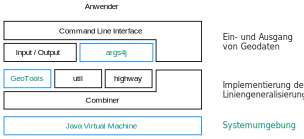
\includegraphics[width=\ScaleIfNeeded]{../chapter5/system-concept}
	\caption{Systemkonzept (schwarz: eigene Entwicklung, blau: benutztes \term{framework})}
	\label{fig:system-concept}
}

Zusammengesetzt ergibt sich aus den besprochenen Aspekten die in Abbildung~\ref{fig:system-concept} dargestellte Architektur:
Dem Anwender steht eine Kommandozeilen-Schnittstelle (CLI) zur Verfügung, die ihrerseits das \term{framework} args4j zum Parsen der Parameter sowie selbst entwickelte Routinen zur Ein- und Ausgabe der Geodaten verwendet.
Die CLI steuert damit die eigentliche Liniengeneralisierung (hier als „Combiner“ bezeichnet), welche ihrerseits neben dem \term{framework} GeoTools noch einige selbst entwickelte Hilfsmodule verwendet, die nicht vom Combiner abhängig sind und deshalb als separates Softwarepaket dargestellt werden (mit „util“ bezeichnet).
Schließlich sitzt zwischen Combiner und CLI ein mit „highway“ bezeichnetes Paket, welches versucht, die Logik des in Abschnitt~\ref{ch:case-selection} ausgewählten Spezialfalls an einem Ort zu bündeln, um die Anpassung auf andere Spezialfälle zu erleichtern.

% Noch mal Modularisierung; java Packages erwähnen/erklären? -> eher nein

Im folgenden Abschnitt wird näher auf die Implementierung der Liniengeneralisierung insbesondere im Combiner eingegangen.



\section{Datenstrukturen}
\label{ch:data-structures}

% - übergeordnete Frage: warum _so_ und nicht anders?

Aus Gründen der Übersichtlichkeit werden in den folgenden Abschnitten nur wesentliche Aspekte und wichtige Entscheidungen behandelt.
Für Detailfragen sei auf die Dokumentation der Programmierschnittstelle verwiesen, welche in englischer Sprache als Teil der Softwareentwicklung im Javadoc-Format angelegt wurde und sowohl im Java-Quellcode als auch im HTML-Format zugänglich ist.

Anhang~\ref{appx:identifiers} löst Bezeichner aus Abschnitt~\ref{ch:algorithm-parts} zu Bezeichnern im Quellcode auf.



\subsection{Grundlegendes Geometrie-Modell (GeoTools)}
\label{ch:data-structures-geotools}

Zur Umsetzung der in Abschnitt~\ref{ch:algorithm-parts} definierten geometrischen Algorithmen werden zunächst Strukturen zur Repräsentation der grundlegenden Datentypen benötigt.
Im Kontext dieses Projekts sind dies:
\begin{enumerate}[nosep]
	\item Punkt (\osm-\term{node})
	\item Segment (Verbindung von zwei Punkten als Teil eines Linienzugs)
	\item Linienzug (\osm-\term{way})
\end{enumerate}

\noindent
Das \term{framework} GeoTools benutzt dazu die JTS Topology Suite, die wie zuvor beschrieben ohnehin wegen des R-Baums für \textproc{NaheSegmente} zum Einsatz kommen soll.
JTS bietet mit der \code{Geometry}-Hierarchie Datenstrukturen nach ISO~19125\hbox{-}1 an, die grundsätzlich auch für die Implementierung der Algorithmen aus Abschnitt~\ref{ch:algorithm-parts} geeignet wären.
% http://atetric.com/atetric/javadoc/com.vividsolutions/jts-core/1.14.0/com/vividsolutions/jts/geom/package-summary.html

Die Algorithmen \textproc{Splitten} und \textproc{Analyse} ordnen den Segmenten allerdings zusätzliche Attribute zu ($wurzel$ bzw. $parallelLinks / parallelRechts$).
Dies unterstützt JTS zwar in Form von \term{user data objects}.
% http://atetric.com/atetric/javadoc/com.vividsolutions/jts-core/1.14.0/com/vividsolutions/jts/geom/Geometry.html#getUserData--
Weil jedoch die Arbeit damit eher umständlich ist, wäre dies nur sinnvoll, wenn die Nutzung der JTS-Datenstrukturen andere Vorteile bietet.

Dies ist jedoch nicht der Fall.
Im Gegenteil passen die JTS-Datenstrukturen nicht gut auf die definierten Algorithmen:
Diese beschränken sich zu einem großen Teil auf Segmente aus exakt zwei Punkten, während JTS von längeren Linienzügen ausgeht.
Die Algorithmen machen sich außerdem zunutze, dass sich Segmente direkt als Vektoren interpretieren lassen (vergleiche Abschnitt~\ref{ch:split-algorithm}).
Routinen zur Vektor-Mathematik bietet JTS zwar grundsätzlich an, jedoch sind wichtige Teile davon nicht spezifiziert.
Beispielhaft sei die Klasse \code{jts.math.Vector2D} genannt, deren Methode \code{angle()} offenbar Winkel berechnet, jedoch in keiner Weise dokumentiert ist.
% http://atetric.com/atetric/javadoc/com.vividsolutions/jts-core/1.14.0/com/vividsolutions/jts/math/Vector2D.html
Die Definition der \textproc{Analyse} auf Parallelität verlangt jedoch einen bestimmten Wertebereich für Winkel von Vektoren.
Obwohl sich die derzeitige Implementierung von \code{angle()} leicht anhand des Quellcodes von JTS ermitteln ließe, ist die Methode nicht zuverlässig verwendbar, weil ohne Dokumentation bereits unklar bleibt, ob die derzeitige Implementierung überhaupt korrekt ist.

Hinzu kommt, dass auch die von JTS angebotenen Operationen zur Manipulation geometrischer Daten -- abgesehen vom räumlichen Index -- hier wenig hilfreich sind.
Ein direktes Verwenden der bereitgestellten JTS-Datenstrukturen erscheint folglich insgesamt betrachtet nicht sinnvoll zu sein.
Stattdessen wurde ein eigenes Datenmodell entwickelt, das im Folgenden beschrieben wird.

JTS bietet die Möglichkeit, das \term{framework} zusammen mit eigenen Datenstrukturen zu benutzten, wenn diese bestimmte Schnittstellen anbieten.
% z. B. CoordinateSequence
% wie in Nr. 8 im "JTS Topology Suite Developer’s Guide" 1.4 beschrieben
Dies käme hier durchaus in Betracht, damit die eigenen Datenstrukturen zukünftig von Dritten unmittelbar mit JTS genutzt werden können.
Beispielsweise könnten so zusammengefasste Linienzüge als Ergebnisse der hier entwickelten Software direkt mit JTS einer Formvereinfachung unterzogen werden.
Weil dies jedoch nicht Bestandteil dieser Arbeit ist und ein Implementieren jener Schnittstellen keinen direkten Nutzen hat, wurde darauf zunächst verzichtet.
Es ließe sich für eine zukünftige Version leicht ergänzen.



\subsection{Grundlegendes Geometrie-Modell (eigene Entwicklung)}

Ein vollständiges Diagramm des entwickelten Datenmodells ist Anhang~\ref{appx:fullpage-model} zu entnehmen.
Vereinfacht auf die grundlegenden Geometrie-Datentypen ergibt sich das in Abbildung~\ref{fig:impl-geometry-model} gezeigte Datenmodell.
Die Segmente sind wie in Abschnitt~\ref{ch:split-algorithm} beschrieben zunächst nicht in den Eingangsdaten vorhanden; sie daraus durch \textproc{Segmentierung} herzustellen, ist jedoch nahezu trivial.

%   https://de.wikipedia.org/wiki/Assoziation_(UML)#Aggregation_und_Komposition

\onefigure{ht}{
% [Dataset]1 <>-- 0…n[Line]1 <>-- 1…n[Segment]1…n <>-- 2[Node]
	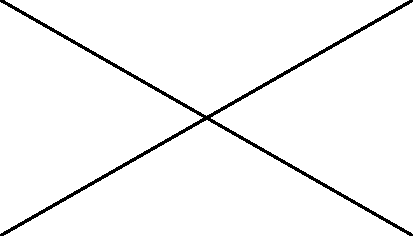
\includegraphics[width=\ScaleIfNeeded]{../image-missing}
	\\\texttt{ [Dataset]<>--[Line]<>--[Segment]<>--[Node]}
	\\\texttt{~~~~~~~~~1~~~0…n~~~1~~~1…n~~~~~1…n~~~2~~~~~}
	\caption{...}
	\label{fig:impl-geometry-model}
}

Die hier gezeigten Datentypen wurden als Interfaces (formale Schnittstellendefinitionen) umgesetzt, um ihre eventuelle Wiederverwendung zu erleichtern. \cf[18]{GHJV95}
Abbildung~\ref{fig:impl-class-structure-splitting} zeigt die bei der Implementierung dieses Datenmodells entstandene Klassenstruktur.

\onefigure{ht}{
% [Klassenstruktur "Splitten"]
	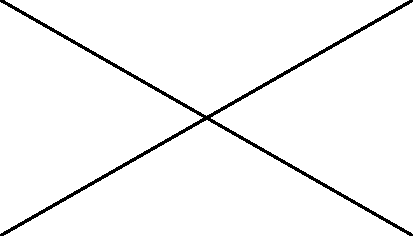
\includegraphics[width=\ScaleIfNeeded]{../image-missing}
	\caption{Klassenstruktur „Splitten“}
	\label{fig:impl-class-structure-splitting}
}

Die Anzahl der jeweils das Interface implementierenden Klassen ist in diesem Projekt klein, so dass es sich anbietet, die jeweiligen Gemeinsamkeiten in abstrakten Klassen
% wie \code{AbstractSegment}
zusammenzufassen, um Redundanzen zu vermeiden.
Diese Klassen gehören daher zu den umfangreicheren im Projekt.
% Herauszustellen ist insbesondere die Klasse \code{AbstractSegment}, welche u.~a. wichtige Algorithmen wie \textproc{Fußpunkt} und \textproc{Analyse} enthält.

Wie in Abschnitt~\ref{ch:split-algorithm} erläutert, existiert derjenige \term{node}, an dem Segmente beim \textproc{Splitten} zerteilt werden, nicht in den Eingangsdaten.
Dementsprechend wird unterschieden zwischen \code{SourceNode} (aus den \osm-Quelldaten kommend) und \code{NonexistentNode} (beim \textproc{Splitten} entstehend).
Beide implementieren jedoch die gemeinsame Schnittstelle für den Typ \code{Node}.
Zu den Gemeinsamkeiten beider Arten von \code{Node}s gehören in erster Linie deren Koordinaten, welche folglich die Klasse \code{AbstractNode} verwaltet und an die beiden konkreten Implementierungen vererbt.

In gleicher Weise fasst \code{AbstractSegment} Gemeinsamkeiten solcher Segmente, die direkt aus den Eingangsdaten stammen (\code{SourceSegment}), und solcher Segmente, die erst durch \textproc{Splitten} eines anderen Segments entstehen (\code{Fragment}), zusammen.
In Abschnitt~\ref{ch:algorithm-parts} wurden solche Segmente zur Vereinfachung einander gleichgestellt.
Für derartige Fälle schlagen Gamma et~al. den Einsatz des Kompositum-Entwurfsmusters vor:
„Use the Composite pattern when [...] you want clients to be able to ignore the difference between compositions of objects and individual objects. Clients will treat all objects in the composite structure uniformly.“ \citex[164]{GHJV95}
Im Kompositum-Muster werden Objekte zu Baumstrukturen aus individuellen Objekten (Blättern) und Komposita von Objekten zusammengefügt.

Im Kontext des Kompositum-Musters ist jedoch die Besonderheit zu berücksichtigen, dass hier einige Blätter aus den Eingangsdaten stammen (\code{SourceSegment}s), andere nicht (\code{Fragment}s).
Gleiches gilt auch für Komposita, so dass sich in einer nur auf Vererbung bestehenden Klassenstruktur sofort eine Wucherung aus größtenteils redundanten Klassen ergäbe.
Für solche Fälle schlagen Gamma et~al. vor, das Brücken-Muster \term{(Bridge pattern)} einzusetzen, mit dem die Redundanz durch Delegation vermieden werden kann. \cf[153]{GHJV95}

\onefigure{ht}{
	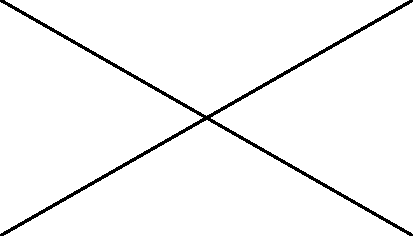
\includegraphics[width=\ScaleIfNeeded]{../image-missing}
	\caption{Composite-Bridge}
	\label{fig:impl-composite-bridge}
}

Eine Kombination aus Kompositum und Brücke wäre zwar möglich, würde jedoch zu einer recht unübersichtlichen Struktur führen.
Gamma et~al. betonen, dass Delegation unweigerlich Komplexität mit sich bringt und nur dann sinnvoll ist, wenn andere Vorteile überwiegen („Delegation is a good design choice only when it simplifies more than it complicates.“ \citex[21]{GHJV95}).
Dies wäre hier offensichtlich nicht der Fall (Abbildung~\ref{fig:impl-composite-bridge}).
Ihre Empfehlung, Delegation möglichst nur in Form von standardisierten Mustern zu verwenden, [\cfibid] scheint hier auch wegen einer weiteren Besonderheit nicht anwendbar zu sein:

Alle Objekte im \code{AbstractSegment}-Kompositum sind veränderbar (\term{mutable}), damit bei der Umwandlung von Blättern (die jeweils ein Segment repräsentieren) in Komposita (die zwei oder mehr Segmente repräsentieren) beim \textproc{Splitten} keine großen Kosten entstehen.
Bloch betont die erheblichen Vorteile von \term{immutability} (\emph{nicht} veränderbarer Objekte), weist aber auch darauf hin, dass bestimmte komplexe Operationen dann sehr teuer werden können („The performance problem is magnified if you perform a multistep operation that generates a new object at every step, eventually discarding all objects except the final result.“ \citex[67]{Blo01}).
Im vorliegenden Kompositum würde \term{immutability} gerade erfordern, dass bei jedem \textproc{Splitten} der Baum neu aufgebaut wird.

Unterschiedliche Klassen für Blätter und Komposita sind deshalb hier gar nicht angebracht; vielmehr bietet es sich \emph{in Anlehnung an} standardisierte Muster an, dass eine gemeinsame Klasse mit einem Attribut \term{children} sich entweder wie ein Blatt oder wie ein Kompositum verhält, je nachdem, ob es \term{children} in Form von Fragmenten gibt oder nicht.

\onefigure{ht}{
	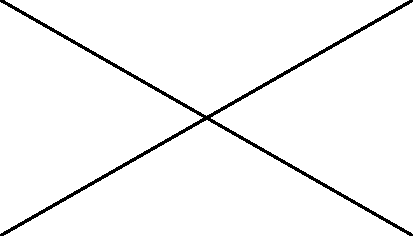
\includegraphics[width=\ScaleIfNeeded]{../image-missing}
	\caption{Composite (IST)}
	\label{fig:impl-class-structure-composite}
}

Aus dieser Erkenntnis ergibt sich eine vergleichsweise einfache Klassenstruktur (Abbildung~\ref{fig:impl-class-structure-composite}):
\code{AbstractSegment} implementiert die Gemeinsamkeiten aller Segmente.
Dazu gehört, dass jedes Segment in genau zwei Fragmente geteilt sein kann, die ihrerseits ebenfalls Segmente sind.
Jedes solche Fragment „weiß“ darüber hinaus, aus welchem Segment es abgetrennt wurde (\term{parent}).

%   [[ Textbausteine:
% In diesem speziellen Fall wird die Struktur der Komposition nur durch SPLITTEN verändert. Dabei wird genau ein Segment durch zwei andere ersetzt, die gemeinsam das ersetzte Segment repräsentieren.
% Dies entspricht zwar dem Composite-Leaf–Modell des Composite-Patterns, aber weil diese Unterscheidung orthogonal zur Unterscheidung in SourceSegment/Fragment ist, 
%   ]]

% TODO:
% soll tatsächliches Objektmodell für Fragmente gezeigt werden oder verwirrt das nur?
% wenn, dann jedenfalls besser nicht vollständig, sondern vereinfacht

Die Unterschiede zwischen \code{SourceSegment} und \code{Fragment} sind zunächst klein.
Die in Abschnitt~\ref{ch:split-algorithm} gegebene Definition von \textproc{NaheSegmente} wurde über den schon erwähnten gepackten R-Baum in JTS implementiert.
Dessen Implementierung hat den Nachteil, dass der so erzeugte R-Baum nach dem Packen nicht mehr verändert werden darf.
% [JTS docs com.vividsolutions.jts.index.strtree.STRtree] (( im Gegensatz zu der Beschreibung in [RSV02 256]! ))
Weil hier ohnehin \code{SourceSegment} als eigene Klasse existiert, bietet es sich an, die \textproc{NaheSegmente}-Logik nur in \code{SourceSegment} zu implementieren statt in der Superklasse \code{AbstractSegment}.
Das Packen des R-Baums braucht dann nur genau einmal nach dem \textproc{Segmentieren} durchgeführt zu werden.
Danach werden die \code{SourceSegment}s nicht mehr verändert.
Da Abschnitt~\ref{ch:split-algorithm} ohnehin eine erneute Abstandsprüfung in der späteren \textproc{Analyse} vorsieht, stellt diese Abweichung von der Definition der Algorithmen nicht die Korrektheit der Implementierung in Frage, obwohl sie mehr Segmente als „nah“ betrachtet als die formale Beschreibung für \textproc{NaheSegmente}.
% (weil SourceSegments obdA größer als Fragments sind). (aber NAHESEGMENTE ist ja primär eine Optimierung)

% TODO:
% Vector erwähnen!

% (weitere Besonderheiten der Konkreten ggü. Abstract*?)
%- SourceNode enthält neben der ID nur Pointers zu den Segmenten etc. für die Korralation
%- SourceSegment außerdem nur L+R sowie analyseLineParts



\subsection{Analyse und Anwendbarkeit auf andere Spezialfälle}
\label{ch:impl-analyser}

Die Algorithmen zur \textproc{Analyse} erfordern die Ergänzung des Datenmodells aus Abbildung~\ref{fig:impl-geometry-model} mit den zusätzlichen Attributen $parallelLinks$ und $parallelRechts$, in denen das Ergebnis der \textproc{Analyse} abgelegt wird.
Wie in Abschnitt~\ref{ch:algorithm-parts} definiert sind dies Attribute des Wurzel-Segments, also der Klasse \code{SourceSegment}.

Obwohl nach der Auswahl eines bestimmten Spezialfalls der Liniengeneralisierung in Abschnitt~\ref{ch:case-selection} andere Fälle nicht weiter berücksichtigt wurden, ist eine auch andere Anwendungsfälle zulassende Flexibilität doch Teil der angestrebten Praxistauglichkeit der zu entwickelnden Software.
Angesichts der Arbeitsweise der Algorithmen ist es naheliegend, dass sich dies insbesondere in der Analyse auf Parallelität niederschlagen sollte.
Die Definition der \textproc{Analyse} beschränkt sich auf geometrische Aspekte; für die konkrete Evaluierung zweiter Segmente spielen im Wesentlichen die Definitionen für \textproc{Parallel}ität und \textproc{Distanz} eine Rolle.
Es wäre daher von Vorteil, wenn diese beiden Definitionen in der Software leicht austauschbar wären.

Dieses Verhalten scheint auf den ersten Blick auf die Beschreibung des Schablonenmethoden"=Entwurfsmusters \term{(Template Method pattern)} zu passen, womit einzelne Schritte verändert werden können, ohne die gesamte Struktur eines Algorithmus zu verändern.
Tatsächlich beschränkt sich dieses Muster jedoch darauf, diese einzelnen Schritte von Unterklassen implementieren zu lassen, was auch in der einleitenden Beschreibung von Gamma et~al. schon deutlich wird:
„Template Method lets subclasses redefine certain steps of an algorithm without changing the algorithm's structure.“ \citex[325]{GHJV95}
Eine Anwendung an dieser Stelle würde also gerade unter Berücksichtigung der oben beschriebenen Komposition von Segmenten in \code{SourceSegment}s und \code{Fragment}s zu einer Wucherung von weiteren Unterklassen führen und wäre daher ungeeignet.

Stattdessen empfehlen Gamma et~al. das Besucher-Muster \term{(Visitor pattern)} einerseits gerade für solche Kompositionen, andererseits gerade dann, wenn wie hier die eigentlichen Datenstrukturen stabil sind, aber doch Flexibilität zur Definition neuer Operationen bieten sollen. \cf[333, 344]{GHJV95}
Dabei erlauben die Objekte der bereits etablierten Datentypen, ihnen einen sog. \term{visitor} als ein unabhängiges Objekt mit definierter Schnittstelle zu übergeben, welches die jeweiligen Operationen implementiert. \cf[331--335]{GHJV95}

In der vorliegenden Software akzeptieren die Segmente den Besuch eines Objekts, das die Schnittstelle \code{Analyser} implementiert.
Dieses Objekt enthält die Implementierungen der Algorithmen \textproc{Parallel} und \textproc{Distanz}.
Im Sinne der besprochenen Systemarchitektur braucht somit das Wissen über das Behandeln des in Abschnitt~\ref{ch:case-selection} gewählten Spezialfalls „baulich getrennte Richtungsfahrbahnen im Straßenraum“ nicht Teil des Combiners zu sein, sondern kann vom Client auf andere Themen angepasst werden.



\subsection{Punktezuordnung}
\label{ch:impl-node-match}

Für Abschnitt~\ref{ch:node-match-algorithm} ergibt sich das in Abbildung~\ref{fig:impl-node-match-model} gezeigte Datenmodell.
Die Klasse \code{NodeMatch} implementiert die Punktezuordnungen.
Dies sind entsprechend der formalen Definition Mengen aus exakt zwei gegenüberliegenden \term{nodes} einander paralleler Segmente.
Die Definition als mathematische Menge zur Vermeidung von Duplikaten wird später beim Zusammenfassen die Interpretation des Begriffs „nächste Zuordnung $c'$“ erleichtern (vergleiche Abschnitt~\ref{ch:generalisation-algorithm}).
Um Objekte der Klasse \code{NodeMatch} klar als Menge zu kennzeichnen, wurde sie zusätzlich als \code{Set<Node>} (Menge von \code{Node}s) im Java Collections Framework deklariert.
Dies erleichtert auch die Implementierung der Mengeneigenschaften.

\onefigure{ht}{
% [NodeGraph]1 <>-- 1…n[NodeMatch]0…n <>-- 2[Node]
	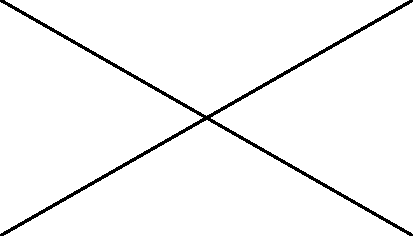
\includegraphics[width=\ScaleIfNeeded]{../image-missing}
	\\\texttt{ [NodeGraph]<>--[NodeMatch]<>--[Node]}
	\\\texttt{~~~~~~~~~~~1~~~1…n~~~~~~~0…n~~~2~~~~~}
	\caption{...}
	\label{fig:impl-node-match-model}
}

Da die \textproc{Analyse} für jedes Segment immer jeweils links- und rechtsseitig nach Parallelen sucht, werden beim \textproc{NodesZuordnen} viele Zuordnungen doppelt gefunden, nämlich einmal in jeder Richtung.
Erneut vereinfachen die Eigenschaften der mathematischen Menge, hier der Menge aller Zuordnungen $C$, die Beschreibung des Algorithmus in Abschnitt~\ref{ch:node-match-algorithm}.
Weil \code{NodeMatch}-Objekte wie beschrieben die Mengeneigenschaften implementieren, können sie leicht direkt im Java Collections Framework verwendet werden, hier als \code{Set<NodeMatch>} (Menge von \code{NodeMatch}-Objekten).
Da der Datentyp \code{NodeMatch} gleichzeitig die Schnittstelle \code{Set<Node>} implementiert, hat die Menge aller Zuordnungen implizit den Typ \code{Set<Set<Node>>}, ist also eine Menge \emph{von Mengen} von \term{nodes}, was genau der formalen Anforderung in Abschnitt~\ref{ch:node-match-algorithm} entspricht.

% TODO: SourceNode, nicht Node. Spielt das eine Rolle, oder versteht man es auch so?

Punktezuordnungen und Segmente ergeben gemeinsamen einen gemischten Graphen des zu generalisierenden Netzes.
Als parallel erkannte Segmente sind über deren \term{nodes} derart einander zugeordnet, dass sich eine gemeinsame Mittellinie als Verknüpfung der Mittelpunkte derjenigen Kanten im Graphen, welche die Punktezuordnungen darstellen, leicht finden lässt.
Zur Definition des Graphen genügt die Menge aller Punktezuordnungen, wenn über die einzelnen Punkte die mit ihnen verknüpften Segmente ermittelbar sind.

% TODO: ist hier der Fall, über addSegment(), welches in AbstractLine passiert. Sollte vielleicht weiter oben in 4.3.1 erwähnt werden. Eventuell könnte auch eine Grafik eines solchen Graphen nicht schaden.



\subsection{Liniengeneralisierung}
\label{ch:impl-generalisation}

Das Ergebnis der Liniengeneralisierung nach Abschnitt~\ref{ch:generalisation-algorithm} ist ein Graph aus Linienzügen, von denen einige durch Zusammenfassen entstehen, andere jedoch mangels Parallelen direkt aus den Eingangsdaten übernommen werden.
Der beschriebene Algorithmus zum \textproc{Zusammenfassen} ergibt einen möglichst langen Linienzug.
Um die spätere Weiterverarbeitung des Generalisierungsergebnisses zu erleichtern, werden hier auch Segmente ohne Parallele zu möglichst langen Linienzügen verkettet.

\onefigure{ht}{
% [GeneralisedLines]1 <>-- 0…n[ResultLine (Section/GeneralisedSection)]0…n <>-- 2…n[Node]
	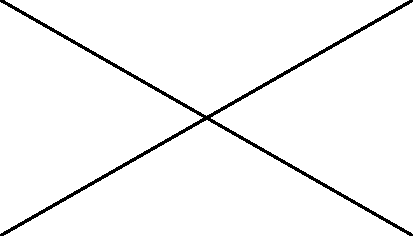
\includegraphics[width=\ScaleIfNeeded]{../image-missing}
	\\\texttt{ [GeneralisedLines]<>--[ResultLine]<>--[Node]}
	\\\texttt{~~~~~~~~~~~~~~~~~~1~~~0…n~~~~~~~~0…n~~2…n~~~~}
	\caption{...}
	\label{fig:impl-generalisation-model}
}

Entsprechend gibt es zwei unterschiedliche Arten von Linienzügen in den Ergebnisdaten.
Dies wird auch vom Datenmodell so abgebildet (Abbildung~\ref{fig:impl-generalisation-model}).
Die Klassen \code{GeneralisedSection} und \code{ConcatenatedSection} enthalten jeweils im Konstruktor Code, dem die Angabe eines geeigneten Startpunkts genügt, um einen Linienzug für das Ergebnis zu bilden.
Die bearbeiteten Segmente werden dabei entsprechend markiert, um doppelte Bearbeitungen zu vermeiden.

Die Klasse \code{GeneralisedSection} enthält den Algorithmus zum \textproc{Zusammenfassen}.
\code{ConcatenatedSection} ist ähnlich aufgebaut, aber wesentlich einfacher, da Punktezuordnungen keine Rolle spielen, sondern nur die jeweils anschließenden Segmente zu berücksichtigen sind.
Beide Klassen sind vom Typ \code{ResultLine}, um dem Client des Combiners einen einheitlichen Typ für die Ergebnisdaten liefern zu können.

Die Klasse \code{GeneralisedLines} ist eine einfache Façade für die Generalisierung, um deren Einsatz zu erleichtern.
% TODO: bessere Beschreibung + GHJV95



\subsection{Integration und ggf. Datenfluss/Interaktionswege \emph{[ausstehend]}}

\begin{itemize}
\item Integration der beschriebenen Klassen zu einem funktionierenden System
\item \code{Combiner} = Façade
\item ggf. Datenfluss/Interaktionswege
% (weichen im imperativen Code teils deutlich von funktional formulierten Algorithmen ab)
\end{itemize}



\section{Schwierigkeiten bei der Umsetzung \emph{[Entwurf]}}
\label{ch:impl-difficulties}

% TODO: "Während der Entwicklung wurde versucht, so viel existierenden Code in Form von \term{frameworks} wiederzuverwenden wie möglich. Diese Bestrebung verursachte Probleme, wie auch später in Abschnitt~\ref{ch:impl-difficulties} geschildert wird."

% TODO: commit log, Notizen und alte Screenshots/Testdaten aufarbeiten

% Wichtig: die Implementierung sollte nur dann nennenswert vom Alg. abweichen, wenn es einen Grund dafür gibt. Der muss dann auch benannt werden.
% Imperfektionen am Alg. sind aber kein Grund, ihn vor Abgabe noch zu verbessern! <= Zeitmangel



\subsection{Eigenschaften der Sprache}

\begin{itemize}

\item
Dass in den zur Verfügung stehenden Java-\term{frameworks} nicht bereits geeignete Datenstrukturen für die Arbeit mit Segmenten existieren, hat einiges an zusätzlicher Arbeit verursacht.
Das Aufbauen der Datenstrukturen war lehrreich, aber zeitaufwändiger als erwartet.

\item
Die Entwicklung von der Idee für einen Algorithmus hin zu einer für komplexe Geodaten praxistauglichen Implementierung kann als iterativer Prozess verstanden werden.
Unter dem Eindruck der Ergebnisse früher Versionen können Algorithmus und Implementierung nach und nach verfeinert werden.
% http://de.wikipedia.org/wiki/Prototyping_(Softwareentwicklung)#Evolution.C3.A4res_Prototyping
Die Wahl von Java als streng typisierte Sprache erschwerte jedoch dieses Vorgehen.
%Der Zeitaufwand dafür, elegante Klassenstrukturen aufzubauen, wurde vom Verfasser unterschätzt.

Die strenge Typisierung hat die Implementierung aufwändiger gemacht und den Fokus (bei vorgegebenem Zeitrahmen für die Arbeit) somit notwendigerweise ein Stück weit verschoben weg von Algorithmusentwicklung und -beurteilung hin zu den Details objektorientierter Programmierung.
Dies war so vor Beginn nicht absehbar.
% denn nur ich+Jochen waren Programmierer, aber nur die offiziellen Betreuer haben akad. Erfahrung
Möglicherweise wäre eine dynamisch typisierte Skriptsprache wie Perl für das explorative Vorgehen geeigneter gewesen.
% warum? -> erfordert Anpassungen der Strukturen von Algorithmen und Daten

\item
Erwartungsgemäß war das Java Collections Framework eine große Hilfe.

\item
Die Idee, nicht nur im Algorithmus, sondern auch in der Typenhierarchie Segmente als Vektoren zu behandeln, stellte sich als sehr hilfreich heraus.
Es ist denkbar, dass eine Sprache mit Operatorüberladung wie Perl diesen Vorteil noch besser hätte ausnutzen können.

\end{itemize}



\subsection{Ein- und Ausgabe von Geodaten}

\begin{itemize}

\item
Zwar ist diese Arbeit ausdrücklich aus \osm\ fokussiert, beim Prototyping stellte sich allerdings heraus, dass das direkten Einlesen von \osm-Daten etwas schwieriger war als erwartet.
Die Eingabe wurde daher zunächst über die Shapefiles der Geofabrik realisiert.
% ein spezielles Shapefile, das zusätzlich die OSM-IDs der Start- und End-Nodes enthält (nur als Debugging-Hilfe; die Algorithmen sind nicht davon abhängig)
Auch die Ausgabe erfolgt zunächst als Shapefile, damit das Generalisierungsergbnis leicht mit gängiger Software betrachtet werden kann.
Schnittstellen für Ein- und Ausgabe von \osm-Daten zu ergänzen, sollte aber nicht allzu schwierig sein.

\item
Die Shapefiles der Geofabrik enthalten aus technischen Gründen veränderte Attribute, nicht die Original-\osm-\term{tags}.
Diesem Problem wurde begegnet, indem ein Adapter die aus den Shapefiles gelesenen Attribute wieder zurück in das \osm-Format wandelt, ohne dass dies für den Combiner sichtbar wird.
% Adapter pattern: io.ShapeTagsAdapter

\item
Die Nutzung des \term{frameworks} GeoTools zur Ein- und Ausgabe von Geodaten war problematisch.
Zwar bietet GeoTools umfangreiche Unterstützung für verschiedene Datenformate, jedoch sind diese I/O-Klassen von GeoTools eher umständlich zu benutzen, ihr Interface ist nicht stabil und sie sind sehr teuer.
Eine Lösung hierfür zu entwickeln, war sehr zeitaufwändig.

Um die Datenausgabe auf eine akzeptable Geschwindigkeit zu beschleunigen, werden diese nun im GeoJSON-Format ausgegeben (implementiert als reine Textausgabe, was sehr billig ist).
Das GeoJSON wird anschließend mit GDAL in ein Shapefile konvertiert.
Insgesamt ist diese Lösung um ein Vielfaches schneller als der Shapefile-Support von GeoTools.

(Allerdings wurde der Shapefile-Support in Geotools neu implementiert; ob dies die Probleme löst, wurde noch nicht getestet.)
% http://web.archive.org/web/20130926213903/http://docs.codehaus.org/display/GEOTOOLS/Migrate+shapefile+to+shapefile-ng

\item
Außer dem eigentlichen Generalisierungsergebnis kann die entwickelte Software auch zahlreiche zusätzliche Geodatensätze ausgeben, die das Verständnis von der Arbeitsweise des Algorithmus bei Anwendung auf Real-World-Daten verbessern und auch beim Debuggen hilfreich sind.
Diese Ausgaben sind in keiner Weise optimiert.

\end{itemize}



\subsection{Sonstiges: Flexibilität und Effizienz}

\begin{itemize}

\label{ch:impl-special-case}
\item
Die Definition des Spezialfalls, auf den die Arbeit beschränkt werden soll, in einem eigenen Paket \code{highway} vom Rest des Combiners zu trennen und sie damit leicht austauschbar zu machen, war grundsätzlich eine gute Idee.
Diese Trennung ist allerdings bisher nur begonnen worden und konnte aus Zeitgründen nicht bis zum Abschluss der Arbeit beendet werden; angesichts der ausdrücklichen Beschränkung in der Aufgabenstellung auf nur den ausgewählten Spezialfall war das aber auch streng genommen gar nicht notwendig.
% betrifft insb. die Klassen Line, AbstractLine, io.InputDataset, io.ShapeReader sowie GeneralisedSection/Section
% "In der vorliegenden Software akzeptieren die Segmente den Besuch eines Objekts, das die Schnittstelle \code{Analyser} implementiert. Dieses Objekt enthält die Implementierungen der Algorithmen \textproc{Parallel} und \textproc{Distanz}." --- stimmt das überhaupt schon?

\item
Im Unterschied zur formalen Definition in Abschnitt~\ref{ch:analyse-algorithm} sind $parallelLinks$ und $parallelRechts$ nicht als homogene binäre Relation auf Segmenten implementiert, sondern als Relation zwischen Segmenten und \emph{Mengen} von Segmenten.
Mit anderen Worten: Es wird nicht jeweils nur ein einziges Segment je Seite als „parallel“ markiert, sondern mehrere.
% es wird in der Tat wie theoretisch überlegt durch die reziproke Zuordnung sichergestellt, dass auch ohne Liste für jedes Paar eine Zuordnung erstellt wird
Auf die Korrektheit der Algorithmen hat dies keinen Einfluss.
Zwar entstehen beim \textproc{NodesZuordnen} zunächst mehr Zuordnungen.
Dies sind jedoch Duplikate, die aufgrund der Mengeneigenschaft entfallen (vergleiche Abschnitt~\ref{ch:impl-node-match}).
Es stellt sich hier also die Frage, welche Implementierungsvariante mit dem Java Collections Framework am effizientesten umzusetzen ist.
Ein \term{profiling} wurde noch nicht durchgeführt.
% => Optimierungspotenzial

\item
Zahllose geschachtelte Schleifen lassen Schlimmes für die Effizienz befürchten, jedoch wird in vielen Fällen nur über eine Menge der Mächtigkeit $2$ iteriert
% (teils weniger, wie die Untersuchung zu realParallels ergab)
und in anderen Fällen wird durch \textproc{NaheSegmente} die Größe der Menge stark begrenzt; deshalb ist der Rechenaufwand in der Praxis gar nicht mal so schrecklich hoch.
Der Speicheraufwand und insbesondere das Verhalten des \term{garbage collectors} ist ein größeres Problem; hier besteht Optimierungspotenzial.

\item
Durchgehende Linienzüge sind in Kapitel~\ref{ch:algorithm-parts} spezifiziert als Mengen zusammenhängender Segmente und sind auch so in \code{AbstractLine} implementiert.
Tatsächlich müssen diese Segmente jedoch für \code{AbstractLine} in jedem Fall erst anhand einer Liste von Stützpunkten erzeugt werden.
Da für \code{ResultLine} die Segmente später ohnehin nur benötigt werden, um daraus gerade eine Liste von Stützpunkten zu erzeugen, wäre eine Optimierung von \code{AbstractLine} durch \term{lazy initialisation} angebracht:
Es würde in \code{AbstractLine} zunächst die Liste von \term{nodes} gespeichert und die \textproc{Segmentierung} erst dann durchgeführt, wenn tatsächlich Segmente angefordert werden.
% Oder es könnte evtl. auch recht einfach ResultLine einige Methoden überschreiben (coordinates, add (-> protected), get/size/iterator etc.)

\end{itemize}



% single-chapter commands
\onlyinsubfile{\listoffigures}
\onlyinsubfile{% UTF-8

\documentclass[../main/thesis.tex]{subfiles}
\begin{document}

% include works in bibliography that aren't cited anywhere in the document (for debugging)
\onlyinsubfile{\nocite{*}}


\defbibnote{thesisBibIntro}{\justify%
Die Literaturangaben sind alphabetisch nach dem Kürzel sortiert.
Das Kürzel wird gebildet aus den ersten drei Buchstaben des Nachnamens des Autors, bei mehreren Autoren aus jeweils den Anfangsbuchstaben der Nachnamen, bei Körperschaften aus einer mnemonisch gewählten Folge von Kleinbuchstaben; jeweils ergänzt durch die letzten beiden Ziffern des Jahres der Veröffentlichung.
\par
Um ein eventuelles Nachschlagen zu erleichtern, sind die Referenzen wo immer möglich durch Angabe von Orten ergänzt, an denen eine Kopie des jeweiligen Werks am 1.~März 2018
% gegen 22~Uhr
aufzufinden war.
In der PDF-Ausgabe dieses Dokuments sind die URLs Hyperlinks.
Die Signaturen beziehen sich auf die Bibliothek des Karlsruher Instituts für Technologie und deren Standort „Fachbibliothek HsKA“.
\bigskip}


\RaggedRight
\addtocontents{toc}{\medskip}
\newpage\addcontentsline{toc}{chapter}{Literaturverzeichnis}
\printbibliography[title=Literaturverzeichnis,prenote=thesisBibIntro]

\end{document}
}
\end{document}

%% UTF-8

% single-chapter commands
\documentclass[../main/thesis.tex]{subfiles}
\onlyinsubfile{\setcounter{chapter}{5}}  % single-chapter command
\begin{document}


\chapter{Ergebnisdiskussion}
\label{ch:result}
% alles NUR im "Anwendungskontext", d.h. in Bezug auf die Ausgabe-Geodaten, nicht die Softwarequalität (das war in 5.4!)

%Die in Kap. 4 und 5 entwickelte Software ist das Ergebnis dieser Arbeit. Hier diskutiert werden soll die Arbeitsweise dieser Software und die Qualität der von ihr ausgegebenen Geodaten in Bezug auf die Aufgabenstellung.

Bei der Evaluierung der Software ist zu bedenken, dass die \osm-Datenbank ständig bearbeitet wird.
Konsistente Ergebnisse für ein bestimmtes Gebiet erfordern dagegen, dass immer mit Geodaten vom selben Stand gearbeitet wird.

In diesem Kapitel wird nach und nach anhand von Einzelbeispielen die Funktion der mit dieser Arbeit entwickelten Software (dem \term{Combiner}) besprochen.
Die genutzten Geodaten für das Straßennetz beschränken sich auf einen Testdatensatz aus \osm\ für das Land Nordrhein-Westfalen vom November~2012.
% http://dev.thaw.de/temp/highways/nrw-roads.zip (testbed-nrw-prepare.sh)

Anhänge~\ref{appx:fullpage-examples-1} und~\ref{appx:fullpage-examples-2} zeigen weitere Beispiele der Anwendung des \term{Combiners} auf aktuelle Geodaten größerer zusammenhängender Areale auch in anderen Regionen.



\section{Anwendung in einfachen Situationen}
\label{ch:result-trivial}

Bei Anwendung des \term{Combiners} auf Geodaten aus der \osm-Datenbank zeigt sich, dass die implementierten Algorithmen grundsätzlich funktionieren.

\onefigure{p}{
	\twofigures{H}{
		\begin{overpic}[width=\ScaleIfNeeded]{../chapter6/result-trivial-in}
			\put(122,84){\figuremark{1}}
			\put(58,60){\figuremark{2}}
			\put(23,39){\rotatebox{50}{\figureframe{.1167}}}
		\end{overpic}
	}{
		\begin{overpic}[width=\ScaleIfNeeded]{../chapter6/result-trivial-out}
			\put(122,84){\figuremark{1}}
			\put(58,60){\figuremark{2}}
			\put(23,39){\rotatebox{50}{\figureframe{.1167}}}
		\end{overpic}
	}
	% trivial = testbed-nrw/koeln-classfied-nolinks.shp
	% 1:30000 Google Mercator, bbox 778765 6607045 780865 6608245, 0.2mm stroke
	\caption{Ergebnis des \term{Combiners} im einfachen Fall (links Eingangsdaten, rechts Generalisierungsergebnis; Köln-Gremberg mit Autobahn L\,124)}
	\label{fig:result-trivial}
}

In Abbildung~\ref{fig:result-trivial} sind links \osm-Linienzüge in der einfachen Situation einer Autobahn ohne Anschlussstellen nebst innerstädtischen Sammelstraßen zu sehen.
Durch Anwendung des \term{Combiners} ergibt sich das rechts dargestellte automatisiert zusammengefasste Ergebnis.
Anstelle der beiden Richtungsfahrbahnen der Autobahn gibt es nun nur noch einen einzigen Linienzug als Straßenachse.
Die Nähe zu nachgeordneten Straßen und deren planfreie Kreuzung mit der Autobahn (bei Markierung~\textfiguremark{1}) stört die Generalisierung nicht.
Auch eine Strecke paralleler Fahrbahnen im nachgeordneten Netz wurde trotz eines scharfen Knicks erfolgreich als parallel erkannt und zusammengefasst (Markierung~\textfiguremark{2}).

\onefigure{p}{
	\twofigures{H}{
		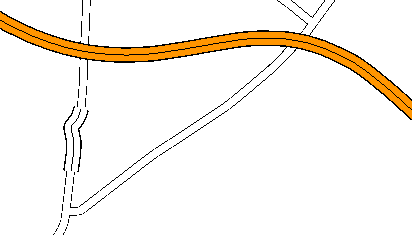
\includegraphics[width=\ScaleIfNeeded]{../chapter6/result-trivial-styled}
	}{
		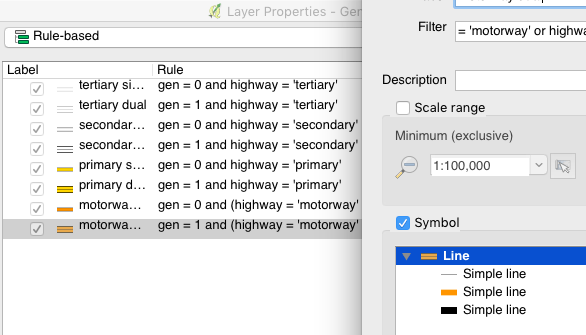
\includegraphics[width=\ScaleIfNeeded]{../chapter6/result-trivial-rules}
	}
	\caption{Visualisierung des Generalisierungsergebnisses (links Kartendarstellung, rechts Screenshot der Zeichenregeln in QGIS)}
	\label{fig:result-trivial-styled}
}

Abbildung~\ref{fig:result-trivial-styled} zeigt beispielhaft, wie sich dieses Generalisierungsergebnis sinnvoll visualisieren ließe.
Der \term{Combiner} kennzeichnet die zusammengefassten Linienzüge als generalisiert.
Zusätzlich gibt der \term{Combiner} einzelne \term{tags} der \osm-Quelldaten mit aus.
Anhand dieser Attribute können leicht Regeln mit jeweils passenden Linearsignaturen definiert werden.

% writeNodeMatches
\onefigure{p}{
	\twofigures{H}{
		\begin{overpic}[width=\ScaleIfNeeded]{../chapter6/result-trivial-detail-rolshover}
			\put(129,0){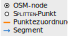
\includegraphics{../chapter6/legend-nodematch}}
			\put(53,7){\figuremark{1}}
			\put(81,85){\figuremark{2}}
			\put(184,83){\figuremark{3}}
		\end{overpic}
	}{
		\begin{overpic}[width=\ScaleIfNeeded]{../chapter6/result-trivial-detail-rolshover-gen}
			\put(129,0){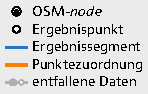
\includegraphics{../chapter6/legend-nodematch-gen}}
			\put(53,7){\figuremark{1}}
			\put(81,85){\figuremark{2}}
			\put(184,83){\figuremark{3}}
		\end{overpic}
	}
	% 1:3500 Google Mercator rotated 50°, bbox 779025 6607525 779270 6607665
	\caption{Detaildarstellung Generalisierung mit Punktezuordnungen (links Eingangsdaten, rechts Generalisierungsergebnis; \textfiguremark{2}~in Abbildung~\ref{fig:result-trivial})}
	\label{fig:result-trivial-detail-rolshover}
}

Bei näherer Betrachtung ist die korrekte Arbeitsweise der implementierten Algorithmen in diesem einfachen Fall gut zu erkennen (Abbildung~\ref{fig:result-trivial-detail-rolshover}):
Linienzüge werden durch \textproc{Splitten} derart unterteilt, dass möglichst jeweils zwei Punkte auf Parallelen einander gegenüber liegen (gut zu sehen bei~\textfiguremark{1}).
Die dabei entstehenden einander gegenüberliegenden Fragmente sind durch ihre Ähnlichkeit offensichtlich einfach auf Parallelität zu prüfen.
Selbst dann, wenn beim \textproc{Splitten} keine optimalen Paare entstehen, gelingt dies, solange wenigstens jeweils ein \emph{Teil} der miteinander verglichenen Segmente zueinander parallel ist (\textfiguremark{2}).
Von den so entstehenden Zuordnungen der einander gegenüberliegenden \osm-\term{nodes} lässt sich durch Verbindung ihrer Mittelpunkte leicht eine Mittellinie im Verlauf der Straßenachse als Ergebnis ableiten.

Der Übergang zwischen generalisierten und nicht generalisierten Linienzügen (\textfiguremark{3}) wird unten im Abschnitt~\ref{ch:relocateGeneralisedNodes} diskutiert.

Für den NRW-Testdatensatz wurden die in Abschnitt~\ref{ch:analyse-algorithm} genannten Beispielwerte von höchstens um $15\degree$ abweichender Ausrichtung und höchstens $\unit[40]{m}$ Abstand zweier \textproc{Parallel}er Segmente empirisch als grundsätzlich tauglich bestätigt.
% evtl. näher ausführen, Tabelle mit Zahlen machen, ...
Für Autobahnen genügt überwiegend bereits ein Limit von nur $10\degree$ Abweichung.
Sonstige Straßen besitzen wesentlich engere Kurvenradien und haben dabei vereinzelt Segmente, welche als parallel gelten könnten, deren Ausrichtung jedoch um $30\degree$ oder mehr voneinander abweicht.

% Ausrichtungsgrenze 15°:
% - empirisch ermittelter vernünftiger Bereich für autobahnähnlich etwa 8..16°
% - empirisch ermittelter vernünftiger Bereich für innerstädtisch etwa 20..40°

% Distanz 40 m:
% - empirisch ermittelter vernünftiger Bereich für autobahnähnlich etwa 40..45 m
% - empirisch ermittelter vernünftiger Bereich für innerstädtisch etwa 35..50 m

Um Praxistauglichkeit zu erreichen, müsste die Definition von \textproc{Parallel} folglich vom Straßentyp abhängen.
Dies wurde aus Zeitgründen nicht mehr als Teil dieser Arbeit umgesetzt.

Der NRW-Testdatensatz enthält als \osmtag{highway}[motorway] attributierte Linienzüge mit einer Gesamtlänge von $\unit[4515]{km}$.
% roads-motorway.shp
Der \term{Combiner} erkennt $\unit[4461]{km}$ davon als parallel; das ausgegebene Ergebnis besteht auf $\unit[97,6]{\%}$ Länge aus zusammengefassten Linienzügen.
Nachdem alle nordrhein-westfälischen Autobahnen zweibahnig ausgebaut sind, wäre bei naiver Betrachtung eine Erkennungsrate von $\unit[100]{\%}$ zu erwarten gewesen.
Die Untersuchung der ausgegebenen Ergebnisdaten hat gezeigt, dass Linienzüge im Wesentlichen in den folgenden Fällen als \emph{nicht} parallel erkannt werden:

\begin{itemize}[nosep]
\item fehlerhafte Klassifizierung von Auf- und Abfahrten (\osmtag{highway}[*])
% (insb. \osmtag{highway}[motorway] statt \term{motorway\_link})
\item fehlerhaftes Attribut für die Straßennummer (\osmtag{ref}[*])
% \osmtag{ref} einseitig fehlend oder voneinander abweichend
\item definierte geometrische Kriterien für Parallelität nicht erfüllt \\(z.~B. ungewöhnlich großer Abstand der Richtungsfahrbahnen)
\end{itemize}
%
Letzteres ist zu erwarten und offensichtlich korrekt.
Die ersten beiden Fälle werden in den folgenden Abschnitten~\ref{ch:result-tags} und~\ref{ch:result-junctions} näher betrachtet.



\section{Berücksichtigung von Attributen}
\label{ch:result-tags}

Die in Abschnitt~\ref{ch:analyse-algorithm} beschriebenen Algorithmen berücksichtigen neben der Klassifizierung der Straße als einziges Attribut die Straßennummer.
% in der Annahme, dass diese normalerweise stimmt
Im NRW-Testdatensatz erkennt der \term{Combiner} $\unit[54]{km}$ der Autobahn-Fahrbahnen nicht als parallel; wird die Straßennummer nicht berücksichtigt, sinkt diese Länge auf $\unit[31]{km}$.

An mehreren der dann neu erkannten Stellen trägt nur eine der beiden Richtungsfahrbahn die Straßennummer als Attribut.
In Abschnitt~\ref{ch:case-selection} wurde dargelegt, dass im Straßennetz grundsätzlich eine vergleichsweise hohe Datenqualität zu erwarten gewesen wäre, weil Fehler darin in der Standard-Karte auf \href{https://www.openstreetmap.org/}{\nolinkurl{osm.org}} störend sichtbar sind und deswegen zügig von \osm-Beitragenden behoben werden.
Die nur für \emph{eine} Richtungsfahrbahn fehlende Straßennummer fällt jedoch dem Beitragenden nicht unbedingt auf, solange die Straßennummer der \emph{anderen} Richtungsfahrbahn korrekt angezeigt wird.

Vereinzelt existieren allerdings sogar widersprüchliche Straßennummern der beiden Richtungsfahrbahnen.
So ist auf mehreren Abschnitten bei Dülmen die eine Fahrbahn \osmtag{ref}[A\,43] gekennzeichnet, die andere jedoch \osmtag{ref}[A\,43;B\,474]; bei Bliesheim trägt eine der Richtungsfahrbahnen der A\,553 das Attribut \osmtag{ref}[A\,1].

Da in diesen Fällen die Geometrie der Fahrbahnen offensichtlich parallel ist, muss hinterfragt werden, welche Bedeutung den Attributen beigemessen werden sollte.
Der \term{Combiner} berücksichtigt derzeit entgegen der ursprünglichen Definition standardmäßig nicht mehr die Straßennummer.
%Auch dies könnte jedoch zu Problemen führen, weil damit zwei Fahrbahnen gleicher Klassifizierung, die nur zufällig parallel sind, jedoch zu unterschiedlichen Straßen gehören, fälschlich als Richtungsfahrbahnen derselben Straße erkannt werden könnten.
Dieses Verhalten kann mit dem Schalter \texttt{--tags} kontrolliert werden.



\section{Verhalten an Straßenkreuzungen}
\label{ch:result-junctions}

\subsection{Beseitigung von Topologielücken}
\label{ch:relocateGeneralisedNodes}

Beim Zusammenfassen von Linienzügen erzeugt der \term{Combiner} neue Stützpunkte entlang einer Mittellinie.
Werden die Stützpunkte der ursprünglichen Linienzüge noch für weitere Zwecke verwendet, dürfen diese nicht entfallen, sondern müssen erhalten bleiben.

% [NZZ12, 14]

An \term{nodes}, die sowohl beim Zusammenfassen entfallene Linien als auch andere Linien benutzen, wird dies zum Problem:
Sie werden von nicht generalisierten Linien weiterbenutzt, die generalisierten Linien hingegen verwenden die neu erzeugten Punkte, so dass an den Übergängen topologische Lücken im Straßennetz entstehen.
Der \term{Combiner} versucht dem zu begegnen, indem die \term{nodes} an den Enden \emph{nicht} generalisierter Linienzüge auf diese Situation hin geprüft und nötigenfalls durch geeignete Punkte auf der generalisierten Mittellinie ersetzt werden.

\onefigure{h}{
	\twofigures{H}{
		\begin{overpic}[width=\ScaleIfNeeded]{../chapter6/koelnarena-gen}
			\put(0,0){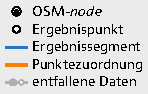
\includegraphics{../chapter6/legend-nodematch-gen}}
			\put(51,67){\figuremark{1}}
			\put(137,24){\figuremark{2}}
		\end{overpic}
	}{
		\begin{overpic}[width=\ScaleIfNeeded]{../chapter6/koelnarena-gen-cleanup}
			\put(0,0){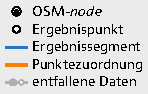
\includegraphics{../chapter6/legend-nodematch-gen}}
			\put(51,67){\figuremark{1}}
			\put(137,24){\figuremark{2}}
		\end{overpic}
	}
	% 1:5500 Google Mercator, bbox 777275 6610050 777660 6610270
	\caption{Detaildarstellung der Beseitigung von Topologielücken (links vorher, rechts nachher; L\,111 in Köln-Deutz)}
	\label{fig:koelnarena-gen-cleanup}
}

Abbildung~\ref{fig:koelnarena-gen-cleanup} zeigt, dass diese Lösung grundsätzlich funktioniert.
Die Straßenkreuzung bei \textfiguremark{1} wird auf einen einzelnen Punkt zusammengefasst, so dass beide Straßen korrekt miteinander verknüpft sind.
Auch der bereits in Abschnitt~\ref{ch:generalisation-algorithm} angesprochene und zunächst offen gelassene Übergang eines einzelnen Linienzugs in zwei parallele Linienzüge bei \textfiguremark{2} wird so gelöst.

Dieses zusätzliche, in Abschnitt~\ref{ch:algorithm-parts} nicht beschriebene Verfahren ist standardmäßig aktiv, kann aber mit dem Schalter \texttt{--no-cleanup} kontrolliert werden.
Auch in Abbildung~\ref{fig:result-trivial-detail-rolshover} kam es zum Einsatz.
Darin ist bei \textfiguremark{3} gut zu sehen, wie am Beginn des generalisierten Abschnitts die Geometrie geringfügig geändert wird, um die Topologie zu erhalten.

Topologielücken können jedoch nur dann mit diesem Verfahren geschlossen werden, wenn tatsächlich ein \emph{geeigneter} Punkt auf der generalisierten Mittellinie gefunden wird.
Wie die folgenden Abschnitte zeigen werden, ist dies oft nicht der Fall.
%Wird ein \emph{un}geeigneter Punkt gefunden, entstehen spitzwinklige Haken (siehe Anhang~\ref{appx:junction-examples}, Abbildung XYZ), Segmente mit Nulllänge usw. usf.

Mit diesem Verfahren können überdies in der gegenwärtigen Implementierung nur solche Topologielücken beseitigt werden, die erst beim Zusammenfassen von Parallelen entstanden sind.
Besonders auffallend ist diese Einschränkung bei Verbindungsrampen an planfreien Kreuzungen.
Sie sind keine Richtungsfahrbahnen und werden deshalb wie in Abschnitt~\ref{ch:case-selection} festgelegt in dieser Arbeit nicht betrachtet.
Sie sind deshalb bereits in den Eingangsdaten für die Zusammenfassung durch Objektauswahl entfallen und damit auch nicht im Generalisierungsergebnis enthalten (Abbildung~\ref{fig:breitscheid-gen-styled}).

Dass einander kreuzende Autobahnen miteinander verknüpft sind, lehrt die Lebenserfahrung; aus der Topologie der generalisierten Geodaten geht es indes nicht hervor.

\onefigure{h}{
	\begin{overpic}[width=7cm]{../chapter6/breitscheid-bg}
		\put(0,0){\scalebox{1}[1.0008]{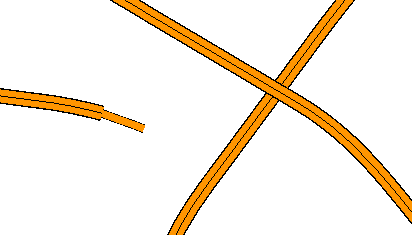
\includegraphics[width=7cm]{../chapter6/breitscheid-gen-styled}}}
	\end{overpic}
	% 1:50000 Google Mercator, bbox 761000 6682100 764500 6684100
	\caption{Fehlende Verbindungsrampen im Generalisierungsergebnis ~~~~~~~~~~~~~~~~~~~~~~~~~\cf[entsättigt][Hintergrund ]{map:osm-carto}}
	\label{fig:breitscheid-gen-styled}
}



\subsection{Fehlende Kreuzungserkennung}
\label{ch:missing-junction-detection}

\onefigure{t}{
	\begin{overpic}[width=\ScaleIfNeeded]{../chapter6/kanal-gen-cleanup}
		\put(0,67.5){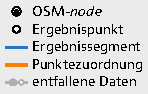
\includegraphics{../chapter6/legend-nodematch-gen}}
		\put(168,35){\figuremark{1}}
		\put(161,85){\figuremark{2}}
		\put(107,33){\figuremark{3}}
	\end{overpic}
	% 1:3500 Google Mercator rotated 10°, bbox 771595 6612098 771840 6612238
	\caption{Verbleibende Topologielücken (Innere Kanalstraße, Köln)}
	\label{fig:kanal-gen-cleanup}
}

Das in Abschnitt~\ref{ch:relocateGeneralisedNodes} beschriebene Verfahren funktioniert auch innerstädtisch nicht in jeder Situation, wie Abbildung~\ref{fig:kanal-gen-cleanup} zeigt.
Zwar führt es zu einem gelungenen Ergebnis bei \textfiguremark{1}.
Bei \textfiguremark{2} und \textfiguremark{3} wird hingegen aufgrund der spezifischen Kreuzungsgeometrie kein „geeigneter“ Punkt auf einer der generalisierten Linien gefunden.
% genauer gesagt: es werden die falschen Punkte gefunden
Die dortigen Lücken in der Topologie bleibt somit bestehen.
Ähnliche Probleme existieren an vielen weiteren innerstädtischen Kreuzungen.

Zwar ließe sich argumentieren, dass in vielen dieser Fälle die Attribute der \osm-Daten fehlerhaft sind.
Beispielsweise sollte in Abbildung~\ref{fig:kanal-gen-cleanup} die \textfiguremark{1} und \textfiguremark{3} verbindende Abbiegefahrbahn eigentlich als solche klassifiziert werden (\osmtag{highway}[primary\_link] statt \term{primary}), wodurch vermieden würde, dass sie bei \textfiguremark{3} als parallel zur Hauptfahrbahn erkannt wird. \cf{osm:HighwayLink}

Allerdings ist gerade dieser Fehler im NRW-Testdatensatz stark verbreitet.
So sind in der Kölner Innenstadt (bis einschließlich der Ringe) von insgesamt 79
% Ringe(außen) + Ringe(mittig) + Ringe(innen) + West + Nord-Süd-Fahrt + Ost:
% 6+13+15+11+26+8
Abbiegefahrbahnen ganze 26
% 2+3+6+5+9+1
nicht als solche klassifiziert.
Es ist auch fraglich, ob hier mit fortschreitender Bearbeitung der \osm-Datenbank Verbesserungen zu erwarten sind, denn Abbiegefahrbahnen und Hauptfahrbahnen werden auf \href{https://www.openstreetmap.org/}{\nolinkurl{osm.org}} mit nahezu identischer Linearsignatur gezeichnet, so dass eine falsche Klassifizierung beim Betrachten nicht auffällt.
% gemeint ist der Effekt, dass crowdgesourcte VGI im Laufe der Zeit zu Korrektheit tendiert
Vor dem Hintergrund der Aufgabenstellung, die das Ziel \emph{praxistauglicher} Algorithmen vorgibt, ist folglich offensichtlich, dass dieses Problem einer automatisierten Lösung bedarf.

An Kreisverkehren gibt es ebenfalls typische Probleme.
Abbildung~\ref{fig:roundabout-gen-cleanup} zeigt, wie alle im Kreis einander gegenüberliegenden Segmente als parallel erkannt werden.
Mit dieser Masse widersprüchlicher Punktezuordnungen kann der Algorithmus zur Zusammenfassung keine brauchbaren Ergebnisse mehr liefern.
Auch der in Abschnitt~\ref{ch:relocateGeneralisedNodes} besprochene Ansatz zur Beseitigung von Lücken in der Topologie läuft ins Leere.

\onefigure{h}{
	\begin{overpic}[width=\ScaleIfNeeded]{../chapter6/roundabout-gen-cleanup}
		\put(0,0){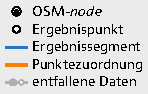
\includegraphics{../chapter6/legend-nodematch-gen}}
	\end{overpic}
	% 1:2000 Google Mercator, bbox 785968 6600972 786108 6601052
	\caption{Verhalten am Kreisverkehr (Friedrichstraße, Köln-Porz)}
	\label{fig:roundabout-gen-cleanup}
}

Zwar wäre es möglich, die meisten Kreisverkehre über \osm-\term{tags} zu erkennen und von der Generalisierung ausschließen (was aber aus Zeitgründen nicht mehr als Teil dieser Arbeit umgesetzt wurde).
% prinzipiell trivial in shouldEvaluate möglich, jedoch erfordert dies, dass die Kreisverkehr-tags vorliegen
Eine Generalisierung der Kreisverkehre -- zum~Beispiel durch Qualitätsumschlag der linearen Kreisfahrbahn in einen einzelnen Kreuzungspunkt im Zentrum -- könnte jedoch überaus nützlich sein, etwa bei der Herstellung einer Straßenkarte im mittleren Maßstabsbereich.

\newpage
Auffallend ist, dass alle diskutierten Probleme an Kreuzungen auftreten.
Auf freier Strecke funktioniert der \term{Combiner} weitgehend problemlos.
Gäbe es eine zuverlässige Methode, automatisiert Kreuzungen zu erkennen, ließe sich möglicherweise leicht Praxistauglichkeit erzielen.

Anhang~\ref{appx:junction-examples} zeigt weitere Beispiele von Kreuzungssituationen, mit denen der \term{Combiner} nicht gut zurechtkommt.



\section{Effizienz}

Die Implementierung der vorgestellten Algorithmen im \term{Combiner} hat bei Anwendung auf den NRW-Testdatensatz wie in Abschnitt~\ref{ch:algorithm-overview} erwartet einen Zeitaufwand, der im Verhältnis zur Zahl der Segmente nicht schneller als linear wächst.
Tabelle~\ref{tab:profiling-segments} stellt die gemessenen Ausführungszeiten $t$ am Beispiel von Fernstraßen (bis einschließlich \osmtag{highway}[primary], ohne \term{links}) in der Umgebung von Köln dar.
% wall clock ("processing time")
Angefangen mit einer Gruppe von Stadtteilen bis hin zum Bundesland Nordrhein-Westfalen wurden steigende Flächengrößen berechnet bei ansonsten gleichen Bedingungen.

\onetable{h}{
	\begin{tabular}{lrrlcccrc}
&&&& \multicolumn{2}{@{}c@{}}{Wachstumsfaktor} &&& \\
Gebiet & \multicolumn{1}{c}{Fläche} & \multicolumn{1}{c}{$|S|$} & \multicolumn{1}{c}{$t$} & für $|S|$ & für $t$ & $\frac{|S'|}{|S|}$ & \multicolumn{1}{c}{$\nu$} & $\psi$ \\
\hline\rule{0mm}{0.8\normalbaselineskip}%
Stadtteile &   161\,km$^2$ &   3516 & 0,41\,s & --  & --  & 1,56 & 10 & 1,31 \\
Großstadt  &   647\,km$^2$ &   8776 & 0,78\,s & 2,5 & 1,9 & 1,48 &  8 & 1,25 \\
Reg.-Bez.  &  7556\,km$^2$ &  54247 & 2,2\,s  & 6,2 & 2,8 & 1,23 &  8 & 1,37 \\
Bundesland & 34881\,km$^2$ & 157014 & 5,7\,s  & 2,9 & 2,6 & 1,27 &  6 & 1,27 \\
	\end{tabular}
	\caption{Zeitbedarf für unterschiedlich große Gebiete}
	\label{tab:profiling-segments}
}

Es bestätigt sich, dass die in Abschnitt~\ref{ch:algorithm-overview} eingeführten Größen $\nu$ und $\psi$ nicht von $|S|$ abhängig sind.
Der Wachstumsfaktor für $t$ beim Schritt von der Großstadt zum Regierungsbezirk ist mit 2,8 deutlich kleiner als der Faktor für $|S|$ mit 6,2 (also besser als für die anderen Schritte).
Wie das Verhältnis $|S'|\nobreak:\nobreak|S|$ der Segmentanzahl nach bzw. vor dem \textproc{Splitten} zeigt, liegt dies an dem mit diesem Schritt erstmals inkludierten ländlichen Raum.
Auch dies entspricht den Erwartungen.

\onetable{b}{
	\begin{tabular}{lcrcccrc}
&&& \multicolumn{2}{@{}c@{}}{Wachstumsfaktor} &&& \\
\term{links} & $|S|$ & \multicolumn{1}{c}{$t$} & für $|S|$ & für $t$ & $\frac{|S'|}{|S|}$ & \multicolumn{1}{c}{$\nu$} & $\psi$ \\
\hline\rule{0mm}{0.8\normalbaselineskip}%
ohne & 54247 & 2,2\,s  & --  & --  & 1,23 &  8 & 1,37 \\
mit & 73408 & 12,8\,s & 1,4 & 5,9 & 1,85 & 11 & 1,42 \\
	\end{tabular}
	\caption{Zeitbedarf ohne und mit Verbindungsfahrbahnen}
	\label{tab:profiling-links}
}

Wird neben der Segmentanzahl in den Eingangsdaten auch deren Detaillierungsgrad geändert, ergibt sich jedoch ein anderes Bild.
Tabelle~\ref{tab:profiling-links} zeigt das Verhalten des \term{Combiners} beim Hinzufügen von Abbiege- und Verbindungsfahrbahnen \term{(links)}.
Der Zeitbedarf wächst hier überproportional.
Dem deutlich gestiegenen Verhältnis $|S'|\nobreak:\nobreak|S|$ zufolge könnte dies an dem bereits in Abschnitt~\ref{ch:impl-special-case} angedeuteten hohen Speicheraufwand der gewählten Implementierung liegen.

Auch dies ist ein deutlicher Hinweis auf die oben diskutierte Notwendigkeit einer Kreuzungserkennung.

% durch Spectre/Meltdown keine großen Einbußen zu erwarten, weil die Berechnung hauptsächlich im RAM stattfindet und somit der Kernel keine große Rolle spielt



\section{Anwendung auf andere Spezialfälle}
\label{ch:result-other-cases}

Der nach Abschnitt~\ref{ch:case-selection} zu untersuchende Spezialfall von \emph{Richtungs}fahrbahnen impliziert, dass die entwickelten Algorithmen genau zwei entgegengerichtete Fahrbahnen derselben Straße zusammenzufassen sollen.
Ebenda wurde jedoch bereits angedeutet, dass sie möglicherweise auch auf andere Spezialfälle anwendbar sein könnten.
Abschließend soll deshalb an zwei Beispielen betrachtet werden, wie sich die im \term{Combiner} implementierten Algorithmen verhalten, wenn die Eingangsdaten nicht entsprechend dem Spezialfall aufgebaut sind, für den die Algorithmen entwickelt wurde.



\subsection{Fahrbahnen für unterschiedliche Arten von Verkehr}
%\label{ch:result-iterated-execution}

Verteilerfahrbahnen und langgezogene Rampen für abbiegenden Verkehr sind verbreitete, schon in Abschnitt~\ref{ch:different-traffic-types-case-desc} genannte Beispiele für parallele Fahrbahnen für unterschiedliche Verkehrsarten.

Nachdem der \term{Combiner} dazu vorgesehen ist, $n$~parallele Linienzüge zu $n-1$~Linienzügen zu generalisieren (mit $n=2$ im Normalfall), liegt es nahe, die Algorithmen zur Generalisierung einfach $n-1$~Mal nacheinander anzuwenden, so dass im besten Fall auch bei beliebig vielen Parallelen am Ende nur noch ein einziger Linienzug übrig bleibt.
Abbildung~\ref{fig:iteration-good} demonstriert, dass diese Strategie gelingen könnte.

\onefigure{h}{
	\twofigures{H}{
		\begin{overpic}[width=\ScaleIfNeeded]{../chapter6/opladen-gen-1}
			\put(0,0){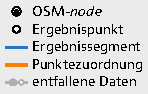
\includegraphics{../chapter6/legend-nodematch-gen}}
		\end{overpic}
	}{
		\begin{overpic}[width=\ScaleIfNeeded]{../chapter6/opladen-gen-2}
			\put(0,0){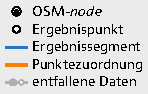
\includegraphics{../chapter6/legend-nodematch-gen}}
		\end{overpic}
	}
	% 1:6500 Google Mercator rotated -24°, bbox 778845 6630050 779300 6630310
	\caption{Detaildarstellung der wiederholten Ausführung für mehr als zwei Parallele (links erste, rechts zweite Generalisierung; A\,3 bei Leverkusen)}
	\label{fig:iteration-good}
}

Wie zu sehen ist, wird in diesem Beispiel die zwischen $2$ und $3$ variierende Zahl von Parallelen in zwei Schritten korrekt auf einen einzelnen Linienzug zusammengefasst.
Dieser liegt allerdings nicht mehr mittig im Verlauf der Straßenachse, sondern ist jeweils seitlich in Richtung der dritten Parallele verschoben.
Eine praxistaugliche Lösung müsste wie in Abschnitt~\ref{ch:generalisation-algorithm} schon angedeutet den Graphen aus Punktzuordnungen und Segmenten in seiner gesamten Breite in nur \emph{einem} Schritt beurteilen, um anhand von Attributen die tatsächliche Straßenachse ermitteln zu können.
Attribute können vom \term{Combiner} bei wiederholter Ausführung gegenwärtig nicht sinnvoll berücksichtigt werden.

Nicht unerwähnt bleiben darf, dass sich das Unvermögen des in Abschnitt~\ref{ch:relocateGeneralisedNodes} vorgestellten Ansatzes zur Beseitigung von Topologielücken, in allen Situationen einen „geeigneten“ Punkt für den Lückenschluss zu finden, bei wiederholter Ausführung besonders stark negativ auf das Ergebnis auswirkt.
Wie Abbildung~\ref{fig:iteration-gaps} zeigt, kommt es vor, dass das Generalisierungsergebnis nach mehreren Wiederholungen mit zahllosen Lücken durchsetzt ist.
Dieses Bild zeigt sich sehr verbreitet, womit das Ergebnis ungeeignet zur Weiterverarbeitung ist.

\onefigure{h}{
	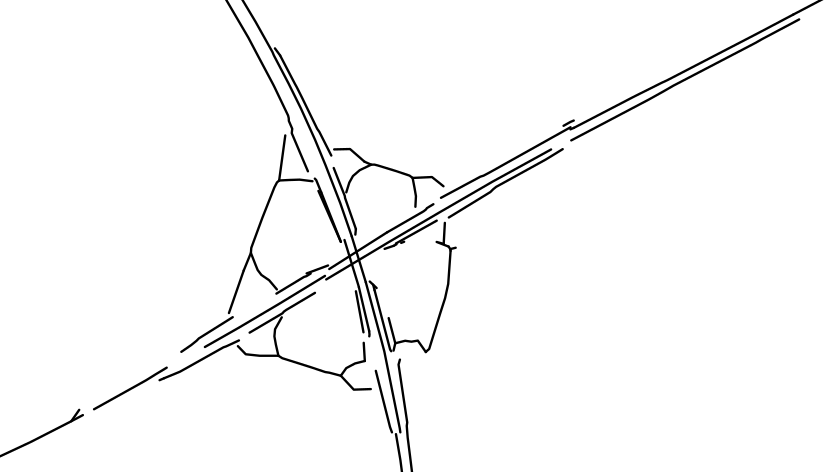
\includegraphics[width=\ScaleIfNeeded]{../chapter6/leverkusen-out}
	\caption{Überreste eines Kleeblatts nach zwei Generalisierungen (Autobahnkreuz Leverkusen)}
	\label{fig:iteration-gaps}
}

Die Anzahl der wiederholt durchzuführenden Generalisierungen kann im \term{Combiner} mit dem Schalter \texttt{--iterations} kontrolliert werden.

% evtl. beidseitig straßenbegleitende Fahrradwege zeigen (nur Erkennung)



\subsection{Eisenbahnstrecken}
\label{ch:result-railways}

Wie sich zeigt, ist die entwickelte Software grundsätzlich auch auf Eisenbahnstrecken anwendbar.
Beschränkt man sich auf Haupt- und Streckengleise (\osmtag{railway}[rail], \osmtag{usage}[main]) und berücksichtigt die Streckennummer als Attribut (\osmtag{ref}[*]), so werden viele doppelgleisige Streckenabschnitte erkannt und zusammengefasst.

Abbildung~\ref{fig:rail-kalk-out} zeigt das Ergebnis der Anwendung auf die südliche Einfahrt zum Güterbahnhof Köln-Kalk (\textfiguremark{1}).
Während die Reisezug-Gleise \textfiguremark{2}--\textfiguremark{3} und auch die drei Zulaufstrecken \textfiguremark{4}, \textfiguremark{5} und \textfiguremark{6} korrekt generalisiert wurden, funktioniert die Zuordnung im Weichenbereich bei \textfiguremark{7} nicht richtig, weil sich hier Gleise mit unterschiedlichen Streckennummern kreuzen.

Dem für ein Straßennetz entwickelten Verfahren zur Beseitigung von Topologielücken aus Abschnitt~\ref{ch:relocateGeneralisedNodes} gelingt es aufgrund der spitzen Winkel nicht, „geeignete“ Punkte zur Beseitigung der Lücken zu finden, wodurch ein gelungenes Ergebnis verhindert wird (Abbildung~\ref{fig:rail-kalk-detail}).

\onefigure{h}{
	\begin{overpic}[width=\ScaleIfNeeded]{../chapter6/rail-kalk-out}
%		\put(0,0){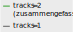
\includegraphics{../chapter6/legend-rail-out}}
	\end{overpic}
	% TODO: QGIS-export, ~10° rotiert
	\caption{Generalisierungsergebnis bei Anwendung des \term{Combiners} auf Bahnstrecken}
	\label{fig:rail-kalk-out}
}
\onefigure{h}{
	\begin{overpic}[width=\ScaleIfNeeded]{../chapter6/rail-kalk-detail}
%		\put(0,0){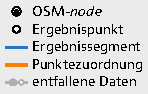
\includegraphics{../chapter6/legend-nodematch-gen}}
	\end{overpic}
	% TODO: QGIS-export, ~60° rotiert
	\caption{Detaildarstellung Generalisierung im Weichenbereich (\textfiguremark{7}~in Abbildung~\ref{fig:rail-kalk-out})}
	\label{fig:rail-kalk-detail}
}

Anders als im Straßennetz existieren derartige Probleme im Eisenbahnnetz nicht nur an Kreuzungen, sondern auch über längere Streckenabschnitte hinweg.
Betroffen sind insbesondere langgestreckte Überwerfungsbauwerke sowie Strecken mit Richtungsbetrieb.
Bei letzteren liegt zwischen den beiden zusammenzufassenden Gleisen mit derselben Streckennummer jeweils ein Gleis einer Strecke mit einer \emph{anderen} Nummer. \cf{wp:Richtungsbetrieb}

Auffallend ist ferner, dass der Zeitbedarf des \term{Combiners} für Bahnstrecken wesentlich höher ist als im Straßennetz.
Für Bahnstrecken in Köln werden mehr als 20~Segmente als „nah“ (im Sinne von \textproc{NaheSegmente} in Abschnitt~\ref{ch:split-algorithm}) beurteilt.
Dies liegt daran, dass Eisenbahngleise oft gebündelt verlegt werden, offenbar um angesichts der großen Kurvenradien den Platzbedarf zu minimieren.
Folglich sind auch entsprechend mehr Teilungen von Segmenten notwendig;
die Annahme $|S'| \approx 2 \cdot |S|$ aus Abschnitt~\ref{ch:algorithm-overview} ist selbst mit der Beschränkung auf Hauptgleise nicht mehr zutreffend.

Tabelle~\ref{tab:profiling-railways} zeigt, dass sich der Zeitbedarf durch bessere Anpassung der Definition von \textproc{Parallel} aus Abschnitt~\ref{ch:analyse-algorithm} auf die Bedingungen im Eisenbahnnetz zumindest geringfügig verbessern lässt.

\onetable{h}{
	\begin{tabular}{lrcrlcccrc}
& \multicolumn{2}{@{}c@{}}{\textproc{Parallel}} &&& \multicolumn{2}{@{}c@{}}{Wachstumsfaktor} &&& \\
Spezialfall & \multicolumn{1}{c}{$\alpha$} & $\eta$ & \multicolumn{1}{c}{$|S|$} & \multicolumn{1}{c}{$t$} & für $|S|$ & für $t$ & $\frac{|S'|}{|S|}$ & \multicolumn{1}{c}{$\nu$} & $\psi$ \\
\hline\rule{0mm}{0.8\normalbaselineskip}%
Straßen    & 15\degree & 40\,m &  8776 & 0,78\,s & --  & -- & 1,48 &  8 & 1,25 \\
Bahngleise & 15\degree & 40\,m & 11607 & 8,2\,s  & 1,3 & 11\hphantom{,2} & 2,81 & 22 & 1,77 \\
Bahngleise &  8\degree & 15\,m & 11607 & 2,5\,s  & 1,3 & \hphantom{1}3,2 & 2,14 & 11 & 1,66 \\
	\end{tabular}
	\caption{Zeitbedarf für unterschiedliche Spezialfälle und \textproc{Parallel}-Definitionen}
	\label{tab:profiling-railways}
}



% evtl. \subsection{Waldschneisen}



% single-chapter commands
\onlyinsubfile{\listoffigures}
\onlyinsubfile{\listoftables}
%\onlyinsubfile{% UTF-8

\documentclass[../main/thesis.tex]{subfiles}
\begin{document}

% include works in bibliography that aren't cited anywhere in the document (for debugging)
\onlyinsubfile{\nocite{*}}


\defbibnote{thesisBibIntro}{\justify%
Die Literaturangaben sind alphabetisch nach dem Kürzel sortiert.
Das Kürzel wird gebildet aus den ersten drei Buchstaben des Nachnamens des Autors, bei mehreren Autoren aus jeweils den Anfangsbuchstaben der Nachnamen, bei Körperschaften aus einer mnemonisch gewählten Folge von Kleinbuchstaben; jeweils ergänzt durch die letzten beiden Ziffern des Jahres der Veröffentlichung.
\par
Um ein eventuelles Nachschlagen zu erleichtern, sind die Referenzen wo immer möglich durch Angabe von Orten ergänzt, an denen eine Kopie des jeweiligen Werks am 1.~März 2018
% gegen 22~Uhr
aufzufinden war.
In der PDF-Ausgabe dieses Dokuments sind die URLs Hyperlinks.
Die Signaturen beziehen sich auf die Bibliothek des Karlsruher Instituts für Technologie und deren Standort „Fachbibliothek HsKA“.
\bigskip}


\RaggedRight
\addtocontents{toc}{\medskip}
\newpage\addcontentsline{toc}{chapter}{Literaturverzeichnis}
\printbibliography[title=Literaturverzeichnis,prenote=thesisBibIntro]

\end{document}
}
\end{document}


% TODO:
% fig:breitscheid-gen-styled - wie zentrieren und vernünftig umbrechen?
% fig:iteration-good - fehlende Punkte darstellen (als nodes, indem das Ergebnis der ersten Gen. als SHP importiert wird) und splitPts wegnehmen (bringen hier nicht mehr viel; evtl. auch Matches wegnehmen? eher ja.)
% fig:rail-kalk-out: neu
% fig:rail-kalk-detail: neu
% Legenden:
% - fig:result-trivial-detail-rolshover (rechts +splitPts, -nodes)
% - fig:koelnarena-gen-cleanup (+splitPts)
% - fig:kanal-gen-cleanup (+splitPts - oder splitPts hier schon wegnehmen? eher nicht.)
% - fig:iteration-good (unklar - erst Grafik neu)
% - fig:rail-kalk-out (fehlt)
% - fig:rail-kalk-detail (fehlt)

%\chapter{Schlussfolgerung und Ausblick}

\section{Praktische Anwendbarkeit}

\begin{itemize}
	\item abschließende qualitative Gesamtbeurteilung der Arbeit auf Basis der Ergebnisuntersuchung in Bezug auf:
	\begin{itemize}
		\item Praxistauglichkeit
		\item Übertragbarkeit auf andere als die spezifizierten Spezialfälle
		\item Übertragbarkeit auf andere, ähnlich gelagerte, aber nicht identische Fragestellungen (z. B. Generalisierung durch Verdrängen)
		\item evtl. in Relation zu existierenden Lösungsansätzen (-> Analyse)
	\end{itemize}
\end{itemize}


\section{Ungelöste Problemfälle}

\begin{itemize}
	\item vorliegende Algorithmen und vorliegende Software
\end{itemize}


\section{Mögliche Ansätze zur Weiterentwicklung}

\begin{itemize}
	\item nächste Schritte
	\item neue Probleme
\end{itemize}


% Arbeit aus dem alten Standpunkt schreiben! Neuere Forschung etc. hier (und evtl. in Einleitung Kontext erklären) -DGD

% weitere Idee: Graphenanalyse: kleinste Ringe finden und prüfen, ob der umschlossene Raum eine ausreichend schmale und lange Form hat, um als parallel gelten zu können; Kreuzungen erkennen durch Mindestgröße (falls unterschritten, auf einen einzigen node zusammenfassen) [ähnlich Tho05]

%% UTF-8

% single-chapter commands
\documentclass[../main/thesis.tex]{subfiles}
\onlyinsubfile{\setcounter{chapter}{7}}  % single-chapter command
\begin{document}


\chapter{Zusammenfassung}

Das Projekt OpenStreetMap (OSM) hat das Ziel der Erstellung einer freien Geodatenbank auf Basis von \term{volunteered geographic information} (VGI).
Die weitere Verarbeitung und Visualisierung von \osm-Daten läuft in aller Regel voll automatisiert ab.
Sie wird erschwert durch den teilweise sehr hohen Detailreichtum, die daraus folgende Fragmentierung von Linienzügen sowie unvollständige Verknüpfungen zusammenhängender Geodaten wie etwa parallelen Richtungsfahrbahnen über Relationen im Datenmodell.

Eine kartographische Generalisierung von \osm-Daten findet bisher nur in geringstem Umfang statt.
Dies fällt unter anderem bei parallelen Richtungsfahrbahnen auf, deren Straßenachse in \osm\ nicht erfasst ist und bisher auch nicht in zufriedenstellender Weise automatisiert abgeleitet werden kann.
%Hier kommt es verbreitet zu unbefriedigenden Darstellungen wie etwa dem Unterschreiten kartographischer Mindestgrößen sowie Fehlern wie etwa dem Überkreuzen der beiden Richtungsfahrbahnen bei Formvereinfachung.
Ansätze zur automatisierten Zusammenfassung von Linienzügen existieren, sind jedoch auf \osm-Daten nicht gut anwendbar.
Insbesondere können sie Kreuzungssituationen oft nicht ohne besondere Attribute lösen.

Diese Arbeit stellt eine Methode zur Erkennung paralleler Linienzüge auf der Basis eines geometrischen Vergleichs kurzer Fragmente vor.
Linienzüge aus \osm\ werden so lange unterteilt, bis sich Stützpunkte auf Parallelen derart einander gegenüberliegen, dass eine Prüfung auf Parallelität leicht möglich ist.
Die anschließende Zusammenfassung der erkannten Parallelen ist dann einfach zu lösen.
Der Rechenaufwand der entwickelten Algorithmen wächst linear mit der Anzahl der Stützpunkte ($\mathcal{O}(n)$).
% eigentlich linear zur Anzahl der Segmente, aber deren Zahl ist proportional zur Anzahl der Stützpunkte, so dass dies keinen Unterschied macht

Zum Nachweis ihrer Funktionsfähigkeit und zum Test mit \term{real world}--Daten aus \osm\ erfolgte ihre ausführbare Implementierung.
Aufgrund einiger technischer Schwierigkeiten war dies aufwändiger als erwartet.
% was den Fokus ein Stück weit weg von der Kartographie hin zur Informatik verschob
Die mit Java entwickelte Software („Combiner“) hat erhebliches Optimierungspotenzial.

Wie sich zeigt, führt die mit dieser Arbeit entwickelte Methode in vielen Fällen zu einem guten Generalisierungsergebnis.
Jedoch leidet auch diese Methode an erheblichen Problemen in Kreuzungssituationen.
Aus Zeitgründen war es nicht möglich, eine praxistaugliche Lösung für diese Probleme zu finden.

% Attribute könnten hier noch erwähnt werden ... sie waren zwar bisher kein großer Teil der Arbeit, müssten es aber werden, wenn Praxistauglichkeit erreicht werden soll

Auch für andere, parallel entwickelte Methoden neueren Datums wird von ähnlichen Problemen in Kreuzungssituationen berichtet.
Eine offensichtliche Lösung mit allgemeiner Anwendbarkeit für das Problem der Zusammenfassung paralleler Linienzüge zeichnet sich derzeit nicht ab.
Es ist jedoch anzunehmen, dass eine zuverlässige automatisierte Kreuzungserkennung die Zusammenfassung zu einem leicht lösbaren Problem machen würde.
Diese Arbeit benennt dazu mehrere unterschiedliche mögliche Ansätze.



\chapter*{Summary}
\addcontentsline{toc}{chapter}{Summary}

...



% single-chapter commands
\end{document}


\listoffigures
%\listofalgorithms
\listoftables
% unified list: see KOMAscript 135

% global bibliography settings

\nocite{*}  % include works in bibliography that aren't cited anywhere in the document (for debugging)

\setbibpreamble{Die Literaturangaben sind alphabetisch nach den Nachnamen der Autoren sortiert. Bei mehreren Autoren wird nach dem ersten Autor sortiert.\par\bigskip\bigskip}

\bibliography{../references-papers,../references-manual}
%\bibliography{../references-manual}


%\appendix
%\chapter{Glossar}
%\chapter{Abkürzungsverzeichnis}
%\chapter{Software-Dokumentation}

\end{document}
